\documentclass[12pt, a4paper]{article}

\usepackage{lastpage}
\usepackage{mathtools}
\usepackage{xltxtra}
\usepackage{libertine}
\usepackage{amsmath}
\usepackage{amsthm}
\usepackage{amsfonts}
\usepackage{amssymb}
\usepackage{enumitem}
\usepackage{xcolor}
\usepackage[left=1.5cm, right=1.5cm, top=2cm, bottom=2cm, bindingoffset=0cm, headheight=15pt]{geometry}
\usepackage{fancyhdr}
\usepackage[russian]{babel}
% \usepackage[utf8]{inputenc}
\usepackage{catchfilebetweentags}
\usepackage{accents}
\usepackage{calc}
\usepackage{etoolbox}
\usepackage{mathrsfs}
\usepackage{wrapfig}

\providetoggle{useproofs}
\settoggle{useproofs}{false}

\pagestyle{fancy}
\lfoot{M3137y2019}
\rhead{\thepage\ из \pageref{LastPage}}

\newcommand{\R}{\mathbb{R}}
\newcommand{\Q}{\mathbb{Q}}
\newcommand{\C}{\mathbb{C}}
\newcommand{\Z}{\mathbb{Z}}
\newcommand{\B}{\mathbb{B}}
\newcommand{\N}{\mathbb{N}}

\newcommand{\const}{\text{const}}

\newcommand{\teormin}{\textcolor{red}{!}\ }

\DeclareMathOperator*{\xor}{\oplus}
\DeclareMathOperator*{\equ}{\sim}
\DeclareMathOperator{\Ln}{\text{Ln}}
\DeclareMathOperator{\sign}{\text{sign}}
\DeclareMathOperator{\Sym}{\text{Sym}}
\DeclareMathOperator{\Asym}{\text{Asym}}
% \DeclareMathOperator{\sh}{\text{sh}}
% \DeclareMathOperator{\tg}{\text{tg}}
% \DeclareMathOperator{\arctg}{\text{arctg}}
% \DeclareMathOperator{\ch}{\text{ch}}

\DeclarePairedDelimiter{\ceil}{\lceil}{\rceil}
\DeclarePairedDelimiter{\abs}{\left\lvert}{\right\rvert}

\setmainfont{Linux Libertine}

\theoremstyle{plain}
\newtheorem{axiom}{Аксиома}
\newtheorem{lemma}{Лемма}

\theoremstyle{remark}
\newtheorem*{remark}{Примечание}
\newtheorem*{exercise}{Упражнение}
\newtheorem*{consequence}{Следствие}
\newtheorem*{example}{Пример}
\newtheorem*{observation}{Наблюдение}

\theoremstyle{definition}
\newtheorem{theorem}{Теорема}
\newtheorem*{definition}{Определение}
\newtheorem*{obozn}{Обозначение}

\setlength{\parindent}{0pt}

\newcommand{\dbltilde}[1]{\accentset{\approx}{#1}}
\newcommand{\intt}{\int\!}

% magical thing that fixes paragraphs
\makeatletter
\patchcmd{\CatchFBT@Fin@l}{\endlinechar\m@ne}{}
  {}{\typeout{Unsuccessful patch!}}
\makeatother

\newcommand{\get}[2]{
    \ExecuteMetaData[#1]{#2}
}

\newcommand{\getproof}[2]{
    \iftoggle{useproofs}{\ExecuteMetaData[#1]{#2proof}}{}
}

\newcommand{\getwithproof}[2]{
    \get{#1}{#2}
    \getproof{#1}{#2}
}

\newcommand{\import}[3]{
    \subsection{#1}
    \getwithproof{#2}{#3}
}

\newcommand{\given}[1]{
    Дано выше. (\ref{#1}, стр. \pageref{#1})
}

\renewcommand{\ker}{\text{Ker }}
\newcommand{\im}{\text{Im }}
\newcommand{\grad}{\text{grad}}

\lhead{Дифференциальные уравнения}
\cfoot{}
\rfoot{Конспект к экзамену}

\usepackage{graphicx}

\begin{document}

\section*{Основные вопросы}

\subsection*{1. Уравнение с разделяющимися переменными: общее решение, общая схема исследования.}

Уравнение с \textbf{разделенными} переменными имеет вид:
\[X(x)dx + Y(y)dy = 0\]

У него решение имеет вид:
\[\int X(x) dx + \int Y(y)dy = C\]

\begin{proof}
    \[\int X(x) dx + \int Y(y)dy = \int X(x) dx + \int Y(y)y' dx = \int (X(x) + Y(y)y')dx = \int 0dx = C\]
\end{proof}

При этом мы получаем общее решение, когда находим такие \(C\), что ответ \(\in C^1\).

Уравнение с \textbf{разделяющимися} переменными имеет вид:
\[p_1(x)q_1(y)dx + p_2(x)q_2(y)dy = 0\]

Если поделить на \(p_2(x)q_1(y)\), то получим уравнение с разделенными переменными. При этом необходимо убедиться, что мы не делим на ноль.

Если \(\exists y_0 : q_1(y_0) = 0\), то \(y\equiv y_0\) --- решение исходного уравнения. Исключив \(y_0\), мы разбиваем область возможных решений на две подобласти.

Аналогично для \(x\).

После разбиения нужно на каждой области найти решение.

\subsection*{2. Линейное уравнение 1-го порядка: общее решение ЛОУ, общее решение ЛНУ. Метод Лагранжа и метод интегрирующего множителя.}

Линейное уравнение первого порядка это
\[y' = p(x)y + q(x)\]

Если \(q\equiv 0\), то это уравнение \textbf{однородно}, иначе \textbf{неоднородно}.

Общее решение ЛОУ это \(y = Ce^{\int p}, C\in\R\)

\begin{proof}
    Заметим, что \(y\equiv 0\) --- решение. По теореме о единственности оно не является особым. т.к. мы рассматриваем \(p\in C(a, b)\).

    \(\sphericalangle y > 0\).
    \[\frac{dy}{y} = p(x)dx\]
    \[\ln y = \int p(x)dx + C\]
    \[y = e^C e^{\int p(x)dx}\]
    По теореме об общем решении уравнения с разделенными переменными это семейство всех решений исходного уравнения при \(y > 0\).

    Аналогично при \(y < 0\)
\end{proof}

Общее решение ЛНУ это
\[y = \left( C + \int qe^{ -\int p} \right)e^{\int p}\]
\begin{proof}
    Подстановкой легко показать, что это решение. Покажем, что нет других решений.

    Пусть есть решение \(\varphi\) на \((\alpha, \beta)\), не подходящее под искомую формулу.

    Пусть \(x_0 \in (\alpha,\beta)\) и \(\varphi(x_0) = y_0\).

    Функция
    \[C = \left( y_0 e^{ -\int p} - \int q e^{ -\int p} dx\right)\Bigg|_{x = x_0}\]

    подходит под искомую формулу, но при этом является решением задачи Коши \(y(x_0) = y_0\), поэтому \(y \equiv \varphi\) --- противоречие.
\end{proof}

\textbf{Метод Лагранжа \textit{(вариации произвольной постоянной)}} --- постоянную \(C\) считают функцией от \(x\) и получают дифур относительно \(C\).

\subsection*{3. Равностепенно непрерывные функции. Лемма Арцела–Асколи.}

Множество функций \(F \), определенных на \(D\), \textbf{равностепенно непрерывно}, если:
\[\forall \varepsilon > 0 \ \ \exists \delta > 0 \ \ \forall f\in F \ \ \forall x_1, x_2\in D \ \ |x_2 - x_1|< \delta \Rightarrow |f(x_2) - f(x_1)|< \varepsilon\]

\begin{lemma}
    Пусть функции последовательности \(\{f_n\}_{n = 1}^{\infty}\) равномерно ограничены \textit{(\(\exists C : \forall n, x |f_n(x)| < C\))} и равностепенно непрерывны на \([a, b]\). Тогда из нее можно выделить подпоследовательность, равномерно сходящуюся на \([a, b]\).
\end{lemma}
\begin{proof}
    Пусть \(M\) ограничивает \textit{(равномерно)} \(f_n\):
    \[M : = \sup_{n, x} |f_n(x)|\]
    \[\sphericalangle \varepsilon_k = \frac{M}{2^{k + 1}}\]
    \[\forall \varepsilon_k > 0 \ \ \exists \delta_k > 0 \ \ \forall f\in F \ \ \forall x_1, x_2\in D \ \ |x_2 - x_1|< \delta_k \Rightarrow |f(x_2) - f(x_1)|< \varepsilon_k\]

    Поделим всю область \([a, b] \times ( - M, M)\) на прямоугольники со стороной \(\varepsilon_1\) и \(\delta_1\).

    Рассмотрим первый столбец. Возьмём два произвольных соседних прямоугольника, таких что по ним проходит бесконечное число \(f\). Вырежем все \(f\), которые по этим прямоугольникам не подходят. Сделаем то же самое для каждого столбца. Получим в итоге \textit{(бесконечную)} подпоследовательность \(F^*_1\).

    Повторим то же самое для всех \(\varepsilon_n, \delta_n\).

    \[\forall f, g\in F^*_i \ \ \forall x\in[a, b] \ \ |f(x) - g(x)| < 2 \varepsilon_n\]
    Нам нужно показать, что \(\forall \varepsilon > 0 \ \ \forall N, k \ \ \forall x\in[a, b] \ \ |f^*_N(x) - f^*_{N + k}(x)|< \varepsilon\)

    Тогда возьмём \(N : 2 \varepsilon_N < \varepsilon\) и все получится, т.к. \(F^*_N \supset F^*_{N + k}\)
\end{proof}

\subsection*{4. ЗК для нормальной системы. Лемма о равносильном интегральном уравнении. Лемма: свойства ломаной Эйлера, определённой на отрезке Пеано.}

Задача Коши для нормальной системы --- нахождение решения, подходящего под условие \(r(t_0) = r_0\)

\(f : \R^{n + 1} \to \R^n\), тогда \(\varphi\) --- решение на \([a, b]\) интегрального уравнения
\[r(t) = r_0 + \int_{t_0}^t f(\tau, r(\tau)) d\tau\]
, если:
\begin{enumerate}
    \item \(\varphi\in C([a, b] \to \R^n)\)
    \item \(\varphi(t) \equiv r_0 + \int_{t_0}^{t} f(\tau, \varphi(\tau)) d\tau\) на \([a, b]\)
\end{enumerate}

\begin{lemma}
    \(\varphi\) --- решение задачи Коши \(\dot r = f(t, r), r\) эквивалентно тому, что \(\varphi\) --- решение
    \[r(t) = r_0 + \int_{t_0}^t f(\tau, r(\tau)) d\tau\]
\end{lemma}
\begin{proof}\itemfix
    \begin{itemize}
        \item [\( \Rightarrow \)] Проинтегрируем \(\dot \varphi(t) = f(\tau, \varphi(\tau))\) от \(t_0\) до \(t\)
        \item [\( \Leftarrow \)] Продифференцируем интегральное уравнение.
    \end{itemize}
\end{proof}

\begin{definition}[Отрезок Пеано]
    \(G\subset \R^{n + 1}_{t, r}\) --- область, \((t_0, r_0)\in G\). Т.к. \(G\) открыто, \(\exists a, b > 0\), такие что параллелепипед с центром в \((t_0, r_0)\) и сторонами \(a, b\) (\(|t - t_0| \leq a, |r - r_0| \leq b\)) лежит в \(G\).

    По теореме Вейерштрасса на компакте есть максимум, т.е. \(\exists M = \max\limits_{\Pi} |f|\). Пусть \(h = \min \{a, \frac{b}{M}\} \). Тогда отрезок \([t_0 - h, t_0 + h]\) --- \textbf{отрезок Пеано}
\end{definition}

Рассмотрим некоторый отрезок Пеано и поделим его правую часть на \(N\) равных частей точками \(t_k\).

Пусть ломаная Эйлера \(E_N\) определена рекурсивно:
\begin{enumerate}
    \item \(E_N(t_0) = r_0\)
    \item \(E_N(t) = E_N(t_k) + f(t_k, E_N(t_k))(t - t_k)\), если \(t\in(t_k, t_{k+1}]\)
\end{enumerate}

\begin{lemma}
    \(\forall t\in[t_0, t_0 + h]\):
    \begin{enumerate}
        \item \(\exists E_N(t)\)
        \item \(|E_N(t) - r_0| \leq M(t - t_0)\), т.е. оно лежит в треугольнике.
    \end{enumerate}
\end{lemma}
\begin{proof}
    Докажем по индукции, что это верно при \(t\in[t_0, t_k]\) для всех \(k\).

    При \(k = 1\) \(E_N\) действительно определена, т.к. \(E_N(t) = r_0 + f(t_0, r_0)(t - t_0)\)

    \[|E_N(t) - r_0| = |f(t_0, r_0)(t - t_0)| \leq M(t - t_0)\]

    Переход индукции:
    \[|E_N(t_k) - r_0| \leq M(t_k - t_0) \leq Mh \leq M \frac{b}{M} = b\]
    Таким образом мы лежим в \(\Pi\), все определено.

    \[|E_N(t) - r_0| = |E_N(t) - E_N(t_0)| \leq |E_N(t) - E_N(t_0)| + |E_N(t_k) - E_N(t_0)| \leq\]
    \[|f(t_k, E_N(t_k))|(t - t_k) + M(t_k - t_0) \leq M(t - t_k) + M(t_k - t_0) = M(t - t_0)\]
\end{proof}

\subsection*{5. Теорема Пеано о существовании решения ЗК.}

\begin{theorem}
    \(G\subset \R^{n + 1}_{t, r}\) --- область, \(f\in C(G\to\R^n), (t_0, r_0)\in G\). Тогда задача Коши имеет решение, определенное на отрезке Пеано для \((t_0, r_0)\).
\end{theorem}
\begin{proof}
    Пусть \(t_0 = 0, r_0 = 0\) \textit{(сдвиг координат)}. Пусть \([ - h, h]\) --- искомый отрезок Пеано. Докажем для \([0, h]\), для другой части аналогично. Объединить оба решения можно по лемме о гладкой стыковке решений.

    Построим бесконечную последовательность ломаных Эйлера. Мы знаем, что \(|E_N(t)| \leq b\), т.е. она равномерно ограничена.

    \[|E_N(t_2) - E_N(t_1)| = \left|\int_{t_1}^{t_2} \dot E_N(\tau)d\tau\right| \leq \int_{t_1}^{t_2} |\dot{E}_N(\tau)|dt\]
    Мы знаем, что \(|\dot{E}_N(t)| \leq M\), поэтому:
    \[|E_N(t_2) - E_N(t_1)| \leq \int_{t_1}^{t_2} |\dot{E}_N(\tau)|dt \leq M(t_2 - t_1)\]
    Пусть \(|t_2 - t_1|< \delta\), тогда \(|E_N(t_2) - E_N(t_1)| < M\delta\) и пусть \(\delta = \frac{\varepsilon}{M}\), тогда \(|E_N(t_2) - E_N(t_1)| < \varepsilon\), т.е. \(E_N\) равностепенно непрерывна. По лемме Арцела–Асколи у этой последовательности есть подпоследовательность, равномерно сходящаяся к некоторой функции \(\varphi\). Покажем, что \(\varphi\) --- решение задачи Коши. Для этого достаточно показать, что:
    \[\varphi(t) \equiv \int_0^{t} f(\tau, \varphi(\tau))d\tau \text{ на } [0, h]\]
    Пусть теперь \(E_N\) --- подпоследовательность исходной последовательности.

    По формуле Ньютона-Лейбница для отображений:
    \[E_N(t) = \int_0^t \dot{E}_N(\tau)d\tau\]
    \[\varphi(t) = \lim_{N \to +\infty}\int_0^t \dot{E}_N(\tau)d\tau\]
    Таким образом, надо показать, что
    \[\lim_{N \to +\infty}\int_0^t \dot{E}_N(\tau)d\tau = \int_0^{t} f(\tau, \varphi(\tau))d\tau\]
    Покажем, что
    \[\Delta_N = \left|\int_0^{t} f(\tau, \varphi(\tau))d\tau - \int_0^t \dot{E}_N(\tau)d\tau\right| \to 0\]
    \[\Delta_N \leq \int_0^t |\dot{E}_N(\tau) - f(\tau, \varphi(\tau))|d\tau \leq \int_0^h |\dot{E}_N(\tau) - f(\tau, \varphi(\tau))|d\tau =\]
    \[\sum_{k = 0}^{N - 1} \int_{t_k}^{t_{k+1}} |\dot{E}_N(\tau) - f(\tau, \varphi(\tau))|d\tau = \sum_{k = 0}^{N - 1} \int_{t_k}^{t_{k+1}} |f(t_k, E_N(t_k)) - f(\tau, \varphi(\tau))|d\tau\]
    \(f\) равномерно непрерывна на параллелепипеде, поэтому \(|(t_k, E_N(t_k)) - (\tau, \varphi(\tau))| < \delta \Rightarrow |f(t_k, E_N(t_k)) - f(\tau, \varphi(\tau))| < \varepsilon\)
    \[\int_{t_k}^{t_{k+1}} |f(t_k, E_N(t_k)) - f(\tau, \varphi(\tau))|d\tau < \varepsilon h\]
    Тогда по двойной бухгалтерии \(\Delta_N \to 0\).

    Но мы не доказали, что \(|(t_k, E_N(t_k)) - (\tau, \varphi(\tau))| < \delta\).

    \[|(t_k, E_N(t_k)) - (\tau, \varphi(\tau))| \leq |(t_k, E_N(t_k)) - (t_k, \varphi(t_k))| + |(t_k, \varphi(t_k)) - (\tau, \varphi(t_k))| + |(\tau, \varphi(t_k)) - (\tau, \varphi(\tau))|\]
    \[ = |E_N(t_k) - \varphi(t_k)| + |t_k - \tau| + |\varphi(t_k) - \varphi(\tau)|\]

    При достаточно больших \(N\) все три слагаемых \( < \frac{\delta}{3}\)
\end{proof}

\subsection*{6. Достаточное условие того, что функция удовлетворяет локальному условию Липшица по заданной переменной.}

Пусть \(G\subset \R^{n + 1}_{t, r}\) --- область, \(f\in C(G \to \R^n), f'_r \in M_{m,n}(C(G))\). Тогда \(f\in \text{Lip}_{r, loc}(G)\)

Кроме того, если \(K\subset G\) --- выпуклый компакт, то \(M_1 : = \max\limits_{(t, r)\in K}|f'_r(t, r)|\), то:
\[\forall (t, r_1), (t, r_2)\in K \ \ |f(t, r_2) - f(t, r_1)| \leq nM_1|r_2 - r_1|\]

\begin{proof}
    Докажем, что на выпуклом компакте \(f\in \text{Lip}_r(K)\).

    Зададим \(g(s) = f(t, r_1 + s(r_2 - r_1))\) \textit{(т.к. \(K\) выпуклый, функция везде определена)}

    \[f(t, r_2) - f(t, r_1) = g(1) - g(0) = \int_0^1 g'(s)ds = \int_0^1 f'_r(t, r_1 + s(r_2 - r_1))(r_2 - r_1) ds\]
    По лемме об оценке нормы произведения матриц \textit{(вектор --- тоже матрица)}
    \begin{align*}
        |f(t, r_2) - f(t, r_1)| & \leq \left|\int_0^1 f'_r(t, r_1 + s(r_2 - r_1))(r_2 - r_1) ds\right|     \\
                                & \leq \int_0^1 \left|f'_r(t, r_1 + s(r_2 - r_1))(r_2 - r_1)\right| ds     \\
                                & \leq \int_0^1 n\left|f'_r(t, r_1 + s(r_2 - r_1))| |(r_2 - r_1)\right| ds \\
                                & \leq \int_0^1 nM_1 |(r_2 - r_1)| ds                                      \\
                                & \leq nM_1 |r_2 - r_1|                                                    \\
    \end{align*}
    Тогда константа Липшица \(nM_1\) и искомое выполнено.

    Почему \(f\in \text{Lip}_{r, loc}(G)\)? Потому что можно для каждой точки взять параллелепипед \(K\) \textit{(выпуклый компакт)} вокруг этой точки и тогда в \(Int K\) выполняется условие Липшица.
\end{proof}

\subsection*{7. Достаточное условие того, что функция удовлетворяет глобальному условию Липшица по заданной переменной.}

Пусть \(G\subset \R^{n + 1}_{t, r}\) --- область, \(f\in C(G \to \R^n)\cap \text{Lip}_{r, loc}(G), K\subset G\) --- компакт. Тогда \(f\in \text{Lip}_{r}(K)\)

\begin{proof}
    Докажем от противного. Пусть \(\forall N\in\N \ \ \exists (t_N, r_N), (t_N, \tilde r_N)\in K\), для которых \(|f(t_N, r_N) - f(t_N, \tilde r_N)| > N|r_N - \tilde r_N|\)

    Т.к. \(K\) компакт, то он секвенциальный компакт, т.е. в \((t_N, r_N)\) и \((t_N, \tilde r_N)\) есть сходящиеся подпоследовательности. Пусть они сходятся к \((t, r)\) и \((t, \tilde r)\) соответственно.

    Либо \(r = \tilde r\), либо нет.

    \begin{enumerate}
        \item \(r = \tilde r\)

              \(\exists U(t, r) : f\in \text{Lip}_r(U)\), т.к. \(f\) лок. Липшицева, т.е. \(\exists L : |f(t', r') - f(t', r'')| \leq L|r' - r''|\)

              Пусть \(N > L\), тогда \(|f(t', r') - f(t', r'')| > N|r' - r''| > L|r' - r''|\) --- противоречие.

        \item
              % \begin{figure}[h]
              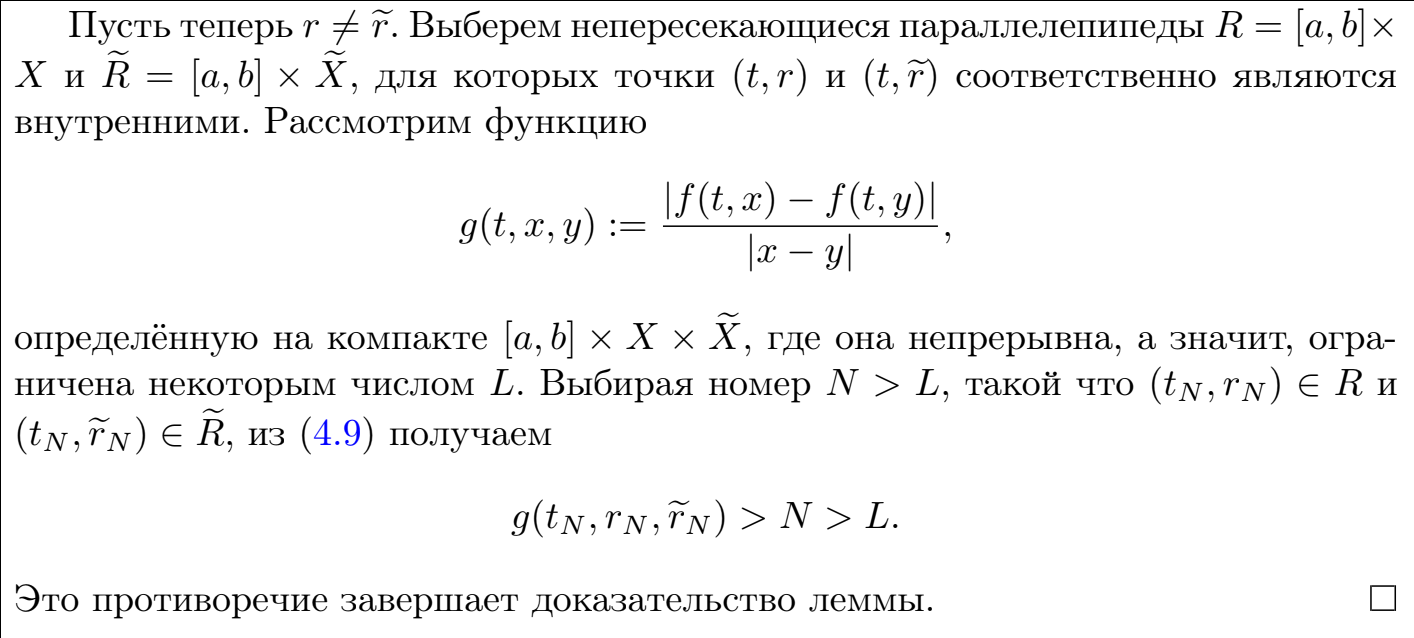
\includegraphics[scale=0.3]{images/7.png}
              %   \end{figure}
    \end{enumerate}
\end{proof}

\subsection*{8. Лемма Гронуолла. Теорема Пикара (доказательство единственности решения).}

\begin{lemma}[Гронуолл]
    \(\varphi\in C[a, b], t_0\in[a, b], \lambda,\mu \geq 0\) и
    \[\forall t\in[a, b] \ \ 0 \leq \varphi(t) \leq \lambda + \mu\left|\int_{t_0}^t \varphi(\tau)d\tau\right|\]
    Тогда
    \[\forall t\in[a, b] \ \ \varphi(t) \leq \lambda e^{\mu|t - t_0|}\]
\end{lemma}
\begin{proof}
    Рассмотрим \(t \geq t_0\) без потери общности.

    Рассмотрим случай \(\lambda > 0\) и пусть \(v(t) = \lambda + \mu\int_{t_0}^t \varphi(\tau)d\tau\). Тогда \(v'(t) = \mu\varphi(t) \leq \mu v(t)\). Таким образом, \(\cfrac{v'(t)}{v(t)} \leq \mu\). Проинтегрировав по \([t_0, t]\), получаем \(v(t) \leq v(t_0)e^{\mu(t - t_0)}\). Таким образом, \(\varphi(t) \leq v(t) \leq v(t_0)e^{\mu(t - t_0)} = \lambda e^{\mu(t - t_0)}\)

    Рассмотрим \(\lambda = 0\), тогда для любого \(\lambda_1\) верно \(\varphi(t) \leq \mu\int_{t_0}^t \varphi(\tau)d\tau < \lambda_1 + \mu\int_{t_0}^t \varphi(\tau)d\tau\), для этого уже доказали.

    При \(\lambda_1 \to 0\) получаем \(\varphi(t) \leq 0\).
\end{proof}

\begin{theorem}
    \(G\subset \R^{n + 1}_{t, r}\) --- область, \(f\in C(G \to \R^n)\cap \text{Lip}_{r, loc}(G), (t_0,r_0)\in G\). Тогда на отрезке Пеано существует решение задачи Коши \(\dot{r} = f(t, r), r(t_0) = r_0\) и оно единственно.
\end{theorem}

\begin{proof}
    Мы доказываем последний пункт, что решение \(\varphi\) единственно.

    Пусть \(\psi_1\) и \(\psi_2\) --- решения на \((a, b)\). По лемме об эквивалентном интегральном уравнении:
    \[\psi_1(t) = \int_0^t f(\tau, \psi_1(\tau))d\tau \quad \psi_2(t) = \int_0^t f(\tau, \psi_2(\tau))d\tau\]
    \[|\psi_1(t) - \psi_2(t)| \leq \int_0^t |f(\tau, \psi_1(\tau)) - f(\tau, \psi_2(\tau))|d\tau\]
    Пусть \([\alpha, \beta]\subset (a, b), a < 0, b > 0\).

    Т.к. графики \(\psi_1\) и \(\psi_2\) на \([\alpha, \beta]\) компактны, \(f(\tau, \psi_1(t))\) и то же самое для \(2\) Липшницевы, поэтому:
    \[|f(\tau, \psi_1(t)) - f(\tau, \psi_2(t))| \leq \tilde L|\psi_1(\tau) - \psi_2(\tau)|\]
    Итого:
    \[|\psi_1(t) - \psi_2(t)| \leq \tilde{L} \int_0^t |\psi_1(\tau) - \psi_2(\tau)|d\tau\]

    По лемме Гронуолла \(|\psi_1(t) - \psi_2(t)|\), т.к. \(\lambda = 0\), таким образом \(\psi_1\) и \(\psi_2\) совпадают на \([\alpha, \beta]\), а в силу произвольности они совпадают и на \((a, b)\)
\end{proof}

\subsection*{9. Теорема Пикара (доказательство существования решения).}

\begin{proof}
    Без потери общности \(t_0 = 0, r_0 = 0\). Рассмотрим правую часть отрезка Пеано \([0, h]\), для левой аналогично и решения можно сшить. Возьмём \(\Pi, M, h\) из определения отрезка Пеано.

    Рассмотрим последовательность функций:
    \begin{itemize}
        \item \(\varphi_0(t) = 0\)
        \item \(\varphi_{k + 1}(t) = \int_0^t f(\tau, \varphi_k(\tau))d\tau\)
    \end{itemize}

    У нас будет три этапа \textit{(в этом билете)}:
    \begin{enumerate}
        \item Докажем, что последовательность верно определена, т.е. \((t,\varphi_k(t))\in G\).
        \item Докажем, что последовательность равномерно сходится на \([0, h]\) к некоторой \(\varphi\)
        \item Докажем, что \(\varphi\) решает интегральное уравнение, эквивалентное искомому.
    \end{enumerate}

    \begin{enumerate}
        \item Докажем по индукции. База тривиальна. Переход:
              \[|\varphi_{k + 1}(t)| \leq \int_0^t |f(\tau, \varphi_k(\tau))|d\tau \leq Mt \leq Mh \leq \frac{Mb}{M} = b\]

        \item Докажем, что \(\forall \varepsilon > 0 \ \ \exists N : \forall t,m > N,k \ \ |\varphi_{m + k}(t) - \varphi_m(t)| \leq \varepsilon\)

              По лемме о достаточном условии Липшица \(f\in \text{Lip}_r(\Pi)\) с константой \(L\). Докажем по индукции, что
              \[|\varphi_{m + k}(t) - \varphi_m(t)| \leq \frac{ML^mt^{m + 1}}{(m + 1)!} \]
              , тогда искомое будет доказано, т.к. \(t < h\) и дробь \( \to 0\).

              База очевидна:
              \[|\varphi_{k}(t) - \varphi_0(t)| \leq \int_0^t |f(\tau, \varphi_{k - 1}(\tau))|d\tau \leq Mt\]

              Переход:
              \begin{align*}
                  |\varphi_{m + 1 + k}(t) - \varphi_{m + 1}(t)|
                   & \leq \int_0^t |f(\tau, \varphi_{m + k}(\tau)) - f(\tau, \varphi_m(\tau))|d\tau \\
                   & \leq \int_0^t L|(\tau, \varphi_{m + k}(\tau)) - (\tau, \varphi_m(\tau))|d\tau  \\
                   & \leq \int_0^t L\frac{ML^m\tau^{m + 1}}{(m + 1)!}d\tau                          \\
                   & \leq \frac{ML^{m + 1}t^{m + 2}}{(m + 2)!}d\tau                                 \\
              \end{align*}
        \item \[\varphi(t) = \lim_{m\to +\infty} \int_0^t f(\tau, \varphi_m(\tau)d\tau\]

              Т.к. \((t, \varphi_m(t))\in \Pi\), то и \((t, \varphi(t))\in \Pi\). Таким образом:
              \[|f(\tau, \varphi_m(\tau)) - f(\tau, \varphi(\tau))| \leq L|\varphi_m(\tau) - \varphi(\tau)|\]
              В силу равномерной сходимости \(\varphi_m\) мы получаем, что \(f(t, \varphi_m(t)) \to f(t, \varphi(t))\) при \(m \to +\infty\) равномерно. Тогда мы можем внести предел под знак интеграла по теореме о предельном переходе под знаком интеграла.
              \[\varphi(t) = \int_0^t f(\tau, \varphi(\tau)d\tau\]
              По лемме об эквивалентном интегральном уравнении получаем, что \(\varphi\) --- решение искомого уравнения.
    \end{enumerate}
\end{proof}

\subsection*{10. Теорема существования и единственности решения ЗК для уравнения $n$-го порядка. Следствие с более простыми условиями.}

\begin{theorem}
    \(G\subset \R^{n + 1}_{t, y, \dot{y}, \dots , y^{(n - 1)}}\) --- область, \(f\in C(G)\), \(f\in \text{Lip}_{(y, \dot{y}, \dots , y^{(n - 1)}), loc}(G), (t_0, y_0, \dot{y}_0, \dots , y^{(n-1)}_0)\in G\). Тогда в некоторой окрестности \(t_0\) есть решение задачи Коши для уравнения \(y^{(n)} = f(t, y, \dot{y}, \dots , y^{(n - 1)})\)
\end{theorem}

\begin{proof}
    Рассмотрим эквивалентную систему. Каждое из уравнений имеет единственное решение задачи Коши по теореме Пикара. По Пикару у эквивалентной системы есть решение.
\end{proof}

\begin{corollary}
    \(G\subset \R^{n + 1}_{t, y, \dot{y}, \dots , y^{(n - 1)}}\) --- область, \(f, f'_y, f'_{y'}, \dots , f'_{y^{(n - 1)}}\in C(G), (x_0, y_0, y_0', \dots , y_0^{(n - 1)})\in G\). Тогда в некоторой окрестности есть единственное решение задачи Коши для уравнения \(y^{(n)} = f(t, y, \dot{y}, \dots , y^{(n - 1)})\).
\end{corollary}

\begin{proof}
    Была лемма, по которой \(f\in \text{Lip}_{(y, \dot{y}, \dots , y^{(n - 1)}), loc}(G)\) и по теореме в этом билете.
\end{proof}

\subsection*{11. Критерий продолжимости.}

\begin{theorem}
    \(G\subset \R^{n + 1}_{t, r}\) --- область, \(f\in C(G \to \R^n)\). Тогда решение \(\varphi\) уравнения \(\dot{r} = f(t, r)\) на промежутке \([a, b)\) продолжимо вправо \(\Leftrightarrow\) \(\exists \lim\limits_{x \to b - 0} \varphi(x) = \tilde{r}\) и при этом \((b, \tilde{r})\in G\)
\end{theorem}

\begin{proof}\itemfix
    \begin{itemize}
        \item [\( \Rightarrow \)] Пусть \(\psi\) --- продолжение вправо \(\varphi\).

              Т.к. \(\psi\) непрерывна, то \(\varphi(b - 0) = \psi(b - 0) = \psi(b)\). Т.к. \(b\in \text{dom}\psi\), \((b, \psi(b))\in G\).

        \item [\( \Leftarrow \)] Доопределим \(\varphi\) на \([a, b]\). На \([a, b)\):

              \[\varphi(t) - \varphi(t_1) = \int_{t_1}^t \varphi'(\tau)d\tau = \int_{t_1}^t f(\tau, \varphi(\tau))d\tau\]

              Пусть \(t_1 \to b\).

              \[\varphi(t) = \tilde{r} + \int_b^t f(\tau, \varphi(\tau))d\tau\]

              По лемме об экв. интегральном уравнении \(\varphi\) --- решение задачи \(\dot{r} = f(t, r), r(b) = \tilde{r}\)

              По теореме Пеано есть решение \(\vartheta\) на \([b - h, b + h]\). Тогда можем сшить \(\vartheta, \varphi\) и получить \(\psi\), это будет решение \([a, b + h]\).
    \end{itemize}
\end{proof}

\subsection*{12. Теорема существования и единственности максимального решения.}

\begin{theorem}
    \(G\subset \R^{n + 1}_{t, r}\) --- область, \(f\in \text{Lip}_{r, loc}(G), f\in C(G \to \R^n), (t_0, r_0)\in G\)

    Тогда максимальное решение задачи Коши существует и единственно.
\end{theorem}
\begin{proof}
    Пусть все решения задачи Коши на интервалах образуют множество \(S\). По теореме Пеано \(|S| \neq 0\). Пусть для \(\varphi\in S\) область определения \((a_\varphi, b_\varphi)\). Пусть \((A,B) : = \bigcup\limits_{\varphi\in S}(a_\varphi, b_\varphi)\)

    Для \(t\in(a_\varphi, b_\varphi)\) пусть \(\psi(t) : = \varphi(t)\). Т.к. все решения задачи Коши совпадают \textit{(теорема Пикара)}, функция задана однозначно. Вполне очевидно, что \(\psi\) --- максимальное решение.

    Другого решения \(\vartheta\) нет, т.к. если \(\text{dom} \vartheta \neq \text{dom} \psi\), то одно из них не максимально, а иначе они равны.
\end{proof}

\subsection*{13. Теорема о выходе интегральной кривой за пределы любого компакта.}

\subsection*{14. Признак продолжимости решения системы, сравнимой с линейной. Теорема о существовании и единственности максимального решения ЛС.}

\subsection*{15. Формула Остроградского–Лиувилля для решений ЛОС.}

\subsection*{16. Общее решение ЛОС. Лемма о множестве фундаментальных матриц. Лемма об овеществлении.}

% \subsection*{17. Теорема о фундаментальной системе решений ЛОС с постоянными коэффициентами (случай жорданова базиса общего вида). Определение и свойства матричной экспоненты (без доказательств). Решение задачи Коши при помощи матричной экспоненты.}

% \subsection*{18. Общее решение ЛНС и метод вариации постоянных.}

% \subsection*{19. Теорема об изоморфизме решений ЛОС и ЛОУ, формула Остроградского–Лиувилля для решений ЛОУ. Метод вариации постоянных для ЛНУ.}

% \subsection*{20. Общее решение ЛОУ с постоянными коэффициентами.}

% \subsection*{21. Теорема об устойчивости ЛОС с постоянными коэффициентами.}

% \subsection*{22. Классификация точек покоя ЛОС 2-го порядка (случай вещественных корней).}

% \subsection*{23. Классификация точек покоя ЛОС 2-го порядка (случай комплексных корней).}

% \subsection*{24. Теорема Ляпунова об устойчивости.}

\section*{Дополнительные вопросы}

\subsection*{Уравнение 1-го порядка и его решение.}

% \begin{definition}
Это уравнение вида \(F(x, y, y') = 0\).
% \end{definition}
% \begin{definition}
Функция \(\varphi\) --- решение такого дифференциального уравнения, если:
\begin{enumerate}
    \item \(\varphi\in C^1(a, b)\)
    \item \(F(x, \varphi(x), \varphi'(x)) \equiv 0\) на \((a, b)\)
\end{enumerate}
% \end{definition}
\begin{example}
    \(y' - x = 0\), решение \(y = \frac{x^2}{2} + C\).
\end{example}

Методов решения много, все относятся к частным случаям.

\subsection*{Интегральная кривая уравнения.}

Это график решения уравнения.

\subsection*{Общее решение уравнения.}

Это множество всех его решений.

\subsection*{Уравнение 1-го порядка, разрешённое относительно производной. Геометрический смысл.}

Это уравнение вида \(y' = f(x, y)\).

Пусть \(\varphi\) решение этого уравнения. Тогда \(\varphi'(x) = f(x, \varphi(x))\), то есть тангенс угла наклона касательной к интегральной кривой в точке \((x_0, y_0)\) это \(f(x_0, y_0)\)

\subsection*{Ломаная Эйлера.}

См. 4

\subsection*{Уравнение в дифференциалах, его решение и параметрическое решение.}

Уравнение в дифференциалах получается, если в уравнении, разрешенном относительно производной, записать \(y' = \frac{dy}{dx} \):
\[P(x, y) dx + Q(x, y) dy = 0\]

Функция \(\varphi\) --- решение такого дифференциального уравнения, если:
\begin{enumerate}
    \item \(\varphi\in C^1(a, b)\)
    \item \(P(x, \varphi(x)) + Q(x, \varphi(x)) \varphi'(x) \equiv 0\) на \((a, b)\)
\end{enumerate}

Аналогично можно определить решение вида \(x = \psi(y)\).

Функция \(r = (\varphi(t), \psi(t))\) --- \textbf{параметрическое} решение такого уравнения на \(\alpha, \beta\), если:
\begin{enumerate}
    \item \(\varphi, \psi\in C^{1}(\alpha, \beta)\) и \(r'(t)\neq 0\) на \(t\in (\alpha, \beta)\)
    \item \(P(\varphi(t), \psi(t)) + Q(\varphi(t), \psi(t))\psi'(t) \equiv 0\) на \(t\in (\alpha, \beta)\)
\end{enumerate}

\begin{example}
    \[xdx + ydy = 0\]

    Подстановкой тривиально можно убедиться, что \(y = \sqrt{C^2 - x^2}\) --- решение этого уравнения.

    Параметрическое решение \((C\cos t, C\sin t)\)
\end{example}

\subsection*{Особые точки уравнения в дифференциалах.}

\((x_0, y_0)\) --- особая, если \(P(x_0, y_0) = Q(x_0, y_0) = 0\)

\begin{example}
    \[xdx + ydy = 0\]

    Особая точка \((0, 0)\), через нее ничто не проходит.
\end{example}

\subsection*{Геометрический смысл уравнения в дифференциалах и его решения.}

Пусть \(r = (x(t), y(t))\) есть параметрическое решение уравнения на \((\alpha, \beta)\). Тогда при \(t\in(\alpha, \beta)\):
\[P(x(t), y(t))x'(t) + Q(x(t), y(t))y'(t) = 0\]
\[F(r(t))r'(t) = 0\]
Таким образом, любая интегральная кривая в каждой своей точке перпендикулярная вектору \(F(x, y)\)

\subsection*{Задача Коши (ЗК) для уравнения 1-го порядка, разрешённого относительно производной.}

Задача Коши --- задача поиска решения уравнения, удовлетворяющему \(y(x_0) = y_0\).

\begin{theorem}
    \(G\subset\R^2\) --- область, \(f\in C(G), (x_0, y_0)\in G\). Тогда в некоторой окрестности \(x_0\) существует решение задачи Коши.
\end{theorem}
\begin{theorem}
    Как в предыдущей теореме, но \(f'_y\in C(G)\). Тогда решение задачи Коши единственно.
\end{theorem}

Таким образом, может быть такое, что в некоторых \textit{(или всех)} точках решение не единственно.

\subsection*{Особое решение уравнения.}

Это решение уравнения, в каждой точке которого нарушается локальная единственность решения задачи Коши.

\begin{example}
    \[y' = \sqrt[3]{y^2}\]
    Тогда особое решение \(y' \equiv 0\), его в любой точке \((x_0, 0)\) пересекает решение вида \(y = (x - x_0)^3 / 3\)
\end{example}

\subsection*{Однородное уравнение.}

Функция однородна степени \(\alpha\), если \(\forall t,x,y \ \ F(tx, ty) = t^\alpha F(x, y)\)

Однородное уравнение --- уравнение вида
\[P(x, y)dx + Q(x, y)dy = 0\]
, где \(P\) и \(Q\) однородные функции одной степени.

Замена \(z = \frac{y}{x}\) сводит это уравнение к уравнению с разделяющимися переменными.

\subsection*{Геометрическое свойство решений однородного уравнения.}

Пусть \(x = \varphi(t), y = \psi(t)\) --- параметрическое решение однородного дифура. Растянем пространство в \(\lambda\) раз, получим \(x = \lambda \varphi(t), y = \lambda \psi(t)\). При подстановке получим:
\[P(\lambda\varphi, \lambda\psi) \lambda\varphi' + Q(\lambda\varphi, \lambda\psi)\lambda\psi' = 0\]
По однородности:
\[P(\varphi, psi) \varphi' + Q(\varphi, \psi)\psi' = 0\]

Таким образом, любое растяжение \textit{(или сжатие)} решения однородного уравнения приводит к другому решению однородного уравнения.

\subsection*{Уравнение Бернулли.}

Это уравнение вида
\[y' = p(x) y + q(x) y^\alpha, \alpha\in\R\setminus \{0,1\}\]

Поделив на \(y^\alpha\) и заменив \(z = y^{1 - \alpha}\), получаем линейное.

\subsection*{Уравнение Риккати.}

\[y' = p(x) y^2 + q(x)y + r(x)\]

Оно решается только в особых случаях \textit{(например, \(\alpha = 2\))}, но если нашел какое-то решение \(\varphi\), то замена \(y = z + \varphi\) сводит к Бернулли.

\subsection*{Уравнение в полных дифференциалах.}

Это уравнение вида
\[P(x, y) dx + Q(x, y)dy = 0\]
, при этом
\[\exists u : du = P(x, y) dx + Q(x, y) dy\]

Решение имеет вид \(u(x, y) = C\)

Обязательное условие на существование \(u\) это \(P'_y = Q'_x\). Если при этом \(P, Q\in C^1(G)\) и \(G\) односвязна, то это условие еще и достаточно.

Если область прямоугольная, то можно решить систему \(\begin{cases}
    u_x' = P \\
    u_y' = Q
\end{cases}\) следующим образом: Решаем первое уравнение при фиксированном \(y\), после чего заменяем \(C = C(y)\) и находим \(C\) как функцию.

В таком случае \(u\) есть потенциал векторного поля \((P, Q)\).

\subsection*{Интегрирующий множитель.}

Это то, на что мы домножаем уравнение, чтобы получить уравнение в полных дифференциалах.

Если \(\mu\) --- инт. множитель, то
\[(\mu P)'_y = (\mu Q)'_x\]
, то есть
\[\mu'_y P - \mu'_x Q = (Q'_x - P'_y) \mu\]

Это сложно решить, но иногда решается при \(\mu'_x \equiv 0\) или \(\mu'_y \equiv 0\).

\subsection*{Уравнение n-го порядка и его решение.}

Это уравнение вида:
\[F(x, y, y', \dots , y^{(n)}) = 0\]

Его решение на \(a, b\) --- \(\varphi\), такое что:
\begin{enumerate}
    \item \(\varphi\in C^n(a, b)\)
    \item \(F(x, \varphi(x), \varphi'(x), \dots , \varphi^{(n)}(x)) \equiv 0\) на \((a, b)\)
\end{enumerate}

\subsection*{ЗК для уравнения, разрешённого относительно старшей производной.}

Это уравнение вида \(y^{(n)} = f(x, y, y', \dots , y^{(n - 1)})\).

Задача Коши для него имеет вид \(y(x_0) = y_0, y'(x_0) = y_1, \dots , y^{(n - 1)}(x_0) = y_{n - 1}\)

\subsection*{Методы понижения порядка уравнения.}

\begin{itemize}
    \item \(y^{(n)} = f(x) \implies y^{(n - 1)} = \int f(x) dx\)
    \item \(F(x, y^{(k)}, y^{(k + 1)}, \dots , y^{(n)}) \xRightarrow{z = y^{(k)}} F(x, z, \dots z^{(n - k)}) = 0\)
    \item \(F(y, y', \dots , y^{(n)}) = 0\). Тогда пусть \(z = y'\), \(y''_{xx} = z'_y z, y'''_{x x x} = z''_{yy} z^2 + z'_y{^2} z\) и т.д.
    \item Пусть \(F\) линейна по \(y\). Тога можно заменить \(z = y'/y\)
    \item \(F(x, y, y', \dots , y^{(n)}) = \cfrac{d}{dx} \Phi(x, y, y', \dots , y^{(n - 1)}) \Rightarrow \Phi(x, y, y', \dots , y^{(n - 1)}) = C\)
\end{itemize}

\subsection*{Нормальная система уравнений, её решение.}

Нормальная система порядка \(n\) это система вида:
\[\begin{cases}
        \dot{x}_1 = f_1(t, x_1, \dots x_n) \\
        \vdots                             \\
        \dot{x}_n = f_n(t, x_1, \dots x_n) \\
    \end{cases}\]

Можно ввести пару обозначений для краткости:
\[r = \begin{pmatrix} x_1 \\ \vdots \\ x_n \end{pmatrix} \quad f(t, r) = \begin{pmatrix} f_1(t, r) \\ \vdots \\ f_n(t, r) \end{pmatrix} \quad \dot{r} = f(t, r)\]

\(\varphi\) --- решение такой системы, если:
\begin{enumerate}
    \item \(\varphi \in C^1((a, b) \to \R^n)\)
    \item \(\dot \varphi(t) \equiv f(t, \varphi(t))\) на \((a, b)\)
\end{enumerate}

\subsection*{Интегральная кривая нормальной системы.}

Это график решения, но теперь он в \((n + 1)\)-мерном пространстве.

\subsection*{Глобальное и локальное условие Липшица.}

Функция \(f : \R^m \to \R^n\) удовлетворяет условию Липшица на множестве \(D\), если \(\exists L\) --- константа Липшица, что для \(\forall r_1, r_2\in D \ \ |f(r_2) - f(r_1)| \leq L|r_2 - r_1|\)

\begin{example}
    Пусть \(f(x) = \sqrt{x}\). Тогда \(f\in \text{Lip}[1 / 2, 1], f\not\in \text{Lip}(0, 1], f\in \text{Lip}_{loc}(0, 1]\)
\end{example}

Функция \(f : \R^{n + 1}_{t, r} \to \R^n\) удовлетворяет условию Липшица по \(r\) \textit{(равномерно по \(t\))} на множестве \(D\), если \(\exists L\), что для \(\forall (t, r_1), (t, r_2)\in D \ \ |f(t, r_2) - f(t, r_1)| \leq L|r_2 - r_1|\), обозначается \(f\in \text{Lip}_r(D)\)

\(f \in \text{Lip}_{loc}(D)\) локально, если \(\forall x_0\in D \ \ \exists U(x_0) \ \ f\in \text{Lip}(U(x_0))\)

\subsection*{Приближения Пикара.}

\begin{itemize}
    \item \(\varphi_0(t) = 0\)
    \item \(\varphi_{k + 1}(t) = \int_0^t f(\tau, \varphi_k(\tau))d\tau\)
\end{itemize}

\subsection*{Сведение уравнения n-го порядка к равносильной системе.}

Пусть \(\Lambda_n y = (y, \dot{y}, \dots , y^{(n - 1)})^T\)

\begin{lemma}
    \(y\) --- решение \(y^{(n)} = f(t, y, \dot{y}, \dots , y^{(n - 1)})\) на \((a, b)\) \(\Leftrightarrow\) \(\Lambda_n y\) --- решение на \((a, b)\) \[\begin{pmatrix} \dot{y}_1 \\ \vdots \\ \dot{y}_{n - 1} \\ \dot{y}_{n} \end{pmatrix} = \begin{pmatrix} y_2 \\ \vdots \\ y_n \\ f(t, y_1, \dots , y_n) \end{pmatrix} \]
\end{lemma}
\begin{proof}\itemfix
    \begin{itemize}
        \item [\( \Rightarrow \)] Пусть \(y\) --- решение первого уравнения. Тогда пусть \(y_k = y^{(k - 1)}\). Тогда первые \(n - 1\) уравнений решаются, а \(\dot{y}_n = y^{(n)} = f(t, y, \dot{y}, \dots , y^{(n - 1)})\), искомое верно.
        \item [\( \Leftarrow \)] Пусть \(r\) --- решение второго уравнения. Будем последовательно дифференцировать первое уравнение и получим искомое.
    \end{itemize}
\end{proof}

\subsection*{Максимальное решение.}

Решение \(\varphi\) продолжимо, если есть решение \(\psi\) на большем отрезке, равное \(\varphi\) на \(\text{dom} \varphi\).

Если у решения нет продолжения, оно максимально.

\subsection*{Определитель Вронского (решений ЛОС и ЛОУ) и его свойства.}

\subsection*{Фундаментальная система решений.}

\subsection*{Фундаментальная матрица.}

\subsection*{Метод неопределённых коэффициентов для ЛС.}

% \subsection*{Характеристический многочлен ЛУ.}

% \subsection*{Метод неопределённых коэффициентов для ЛУ.}

% \subsection*{Автономная система.}

% \subsection*{Фазовое пространство автономной системы. Фазовая траектория, фазовый портрет, фазовая скорость, точка покоя.}

% \subsection*{Устойчивость по Ляпунову и асимптотическая устойчивость.}

% \subsection*{Функция Ляпунова.}

% \subsection*{Теорема об устойчивости по первому приближению.}


\end{document}
